\begin{table}[]
    \begin{tabular}{r|l|r}
    \textbf{Exp. Name} & \textbf{Resources} & \textbf{Total} \\ \hline
    \textbf{A-1,2,3,4,6,8} & \{1, 2, 3, 4, 6, 8\}xUS & 1,2,3,4,6,8\\ \hline
    \textbf{B-2} & 1xUS + 1xEU & 2\\
    \textbf{B-4} & 2xUS + 2xEU & 4\\
    \textbf{B-6} & 4xUS + 2xEU & 6\\
    \textbf{B-8} & 4xUS + 4xEU & 8 \\ \hline
    \textbf{C-3} & 1xUS + 1xEU + 1xASIA & 3\\
    \textbf{C-4} & 1xUS + 1xEU + 1xASIA + 1xAUS & 4\\
    \textbf{C-6} & 2xUS + 2xEU + 2xASIA & 6\\
    \textbf{C-8} & 2xUS + 2xEU + 2xASIA + 2xAUS & 8\\
    \end{tabular}
    \caption{Geo-distributed experiments on GC with T4 VMs.}
    \label{tab:geodistributed-experiments}
    \vspace*{-10mm}
\end{table} 

As spot prices for the same hardware differ depending on the region, zone, and time of day~\cite{lee2017deepspotcloud}, it might be a good idea to use VMs across different data centers.
However, is the connectivity between regions and continents good enough to enable distributed deep learning?
To explore this question, we decided to conduct three types of experiments (\Cref{tab:geodistributed-experiments}):
\begin{description}
    \item[(A) Intra-zone] Can we scale if the VMs are co-located in the same zone (\texttt{us-central-1})?.
    \item[(B) Transatlantic] Can we scale when we combine VMs from two regions (US and EU) across the Atlantic Ocean, and what happens when the compute is unevenly distributed across the regions?
    \item[(C) Intercontinental] Can we scale if we combine VMs from four continents (US, EU, ASIA, AUS)?
\end{description}


\textbf{Experimental design.} 
Based on the insights from ~\Cref{sec:model-suitability}, we decided to use the largest models (ConvNextLarge, RoBERTaXLM) for all further cloud experiments in ~\Cref{sec:geodistributed-performance,sec:multicloud-performance,sec:hybrid-cloud-performance}, with the TBS of 32K as a baseline with good scaling properties.
We abbreviate them with their respective domain names (CV, NLP).
We used Google Cloud~\cite{gcweb} for all experiments in this section, as they were the first to give us access to all necessary zones.
The default networking solution in GC is the "Premium Tier", which tries to use a Google-owned network instead of the public internet.
We measured the throughput and latency between all zones via \texttt{iperf} and \texttt{ping} and report the average of 5 consecutive runs in ~\Cref{tab:geodistributed-network}.
Unsurprisingly, the diagonal shows that the local connectivity between zones runs at almost 7~Gbits with a latency of 0.7ms, probably due to the hypervisors being in the same data center.
While the up- and download were perfectly symmetrical in all setups, the throughput dropped to <210 Mbits for all non-local connections.
The US-based data center is located in Iowa and is best connected with at least 120~Mbits to the remaining regions, namely Belgium in the EU (6,911km), Taiwan in ASIA (11,853km), and Sydney in Australia (AUS, 14,555km), presumably due to the physical distance. 
The lowest bandwidth and highest latency connections are between the EU region and ASIA and AUS, reaching around 80~Mbits and 270ms.
We decided to use the \texttt{n1-standard-8} template with eight cores, 30~GB memory, and a T4 GPU, as the smaller image with 15~GB was insufficient to meet the memory requirements for gradient application on the CPU with the biggest models.
The experiment naming in this section is prefixed with the type of location \textbf{(A)}, \textbf{(B)} or \textbf{(C)} and the number of VMs, e.g., A-4 is the intra-zone experiment with 4 VMs.
The full experimental description is specified in ~\Cref{tab:geodistributed-experiments}.
\vspace*{-2mm}
\begin{table}[h]
    \scalebox{0.6}{
    \begin{subtable}[h]{0.38\textwidth}
        \centering
        \begin{tabular}{l|rrrr}
        \backslashbox{\textbf{From}}{\textbf{To}} & \textbf{US} & \textbf{EU} & \textbf{ASIA} & \textbf{AUS} \\ \hline
        \textbf{US}   & \cellcolor[HTML]{67F13A}6.90 & \cellcolor[HTML]{fadc24}0.21 & \cellcolor[HTML]{fab724}0.13 & \cellcolor[HTML]{fab724}0.12 \\
        \textbf{EU}   & \cellcolor[HTML]{fadc24}0.21 & \cellcolor[HTML]{67F13A}6.81 & \cellcolor[HTML]{fa7e24}0.08 & \cellcolor[HTML]{fa7e24}0.07 \\
        \textbf{ASIA} & \cellcolor[HTML]{fab724}0.13 & \cellcolor[HTML]{fa7e24}0.08 & \cellcolor[HTML]{67F13A}6.79 & \cellcolor[HTML]{fab724}0.16 \\
        \textbf{AUS}  & \cellcolor[HTML]{fab724}0.12 & \cellcolor[HTML]{fa7e24}0.07 & \cellcolor[HTML]{fab724}0.16 & \cellcolor[HTML]{67F13A}6.84 
        \end{tabular}
        \caption{Single stream TCP throughput in Gbits.}
        \label{tab:geodistributed-throughput}
    \end{subtable}
    }
    \scalebox{0.6}{
    \begin{subtable}[h]{0.38\textwidth}
        \centering
        \begin{tabular}{l|rrrr}
        \backslashbox{\textbf{From}}{\textbf{To}}     & \textbf{US} & \textbf{EU} & \textbf{ASIA} & \textbf{AUS} \\ \hline
        \textbf{US}   & \cellcolor[HTML]{67F13A}0.66 & \cellcolor[HTML]{fadc24}103.11 & \cellcolor[HTML]{fab724}157.09 & \cellcolor[HTML]{fab724}176.19 \\
        \textbf{EU}   & \cellcolor[HTML]{fadc24}103.14 & \cellcolor[HTML]{67F13A}0.65 & \cellcolor[HTML]{fa7e24}253.10 & \cellcolor[HTML]{fa7e24}271.98 \\
        \textbf{ASIA} & \cellcolor[HTML]{fab724}157.08 & \cellcolor[HTML]{fa7e24}253.09 & \cellcolor[HTML]{67F13A}0.72 & \cellcolor[HTML]{fab724}131.45 \\
        \textbf{AUS}  & \cellcolor[HTML]{fab724}175.98 & \cellcolor[HTML]{fa7e24}272.08 & \cellcolor[HTML]{fab724}131.42 & \cellcolor[HTML]{67F13A}0.64
        \end{tabular}
        \caption{ICMP latency in ms.}
        \label{tab:geodistributed-ping}
    \end{subtable}
    }
    \caption{Throughput and latency between GC zones.}
    \label{tab:geodistributed-network}
    \vspace*{-8mm}
\end{table}

\textbf{(A) Intra-zone scalability.}
Figure~\ref{fig:geo-dist-us-only} shows the result of the intra-zone experiments, which we used as a baseline to compare geo-distributed deployments to.
As the scalability of the CV and NLP models was already shown with much better hardware and slightly worse network connectivity (cf.~\Cref{sec:model-suitability}), the scalability with the T4 GPUs is not too surprising.
We do not see an improvement in throughput for two GPUs for either model due to the Hivemind penalty discussed in ~\Cref{sec:model-suitability}.
However, starting with three GPUs, we see a steady increase in throughput with a maximum speedup of up to 3.2x CV and 2.75x for NLP at eight GPUs. 
CV's per-GPU speedup ($\frac{\text{speedup}}{\#\text{GPUs}}$) is almost linear (0.43, 0.42, 0.43, 0.41, 0.41), while NLP starts dropping off faster (0.51, 0.47, 0.45, 0.40, 0.34) for 2, 3, 4, 6 and 8 GPUs, respectively.
The reason for this is the NLP granularity of 1.15 with 8 GPUs indicating an almost equal part in communication and calculation (\Cref{fig:geo-dist-us-only-granularity}) due to the much longer averaging round related to the model size (198M vs. 560M parameters).

\begin{figure}
    \begin{subfigure}[c]{0.25\textwidth}
        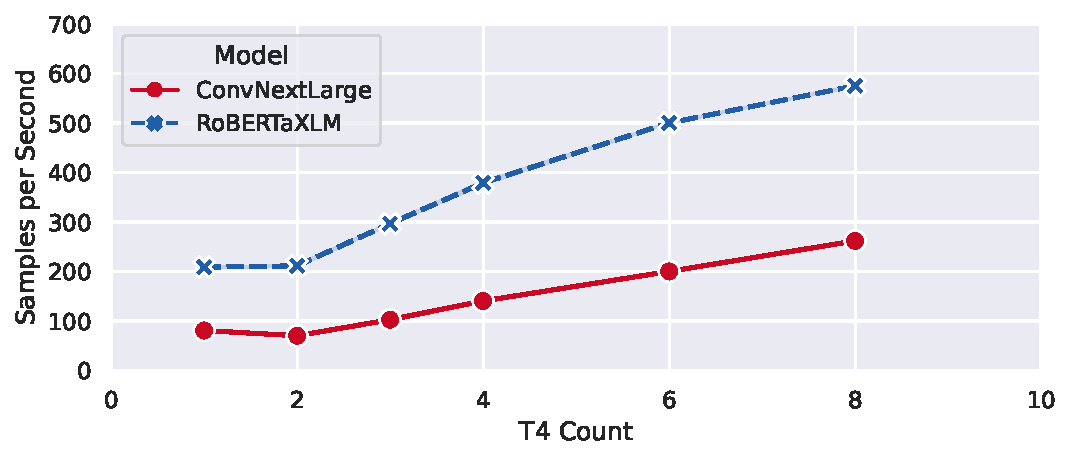
\includegraphics[width=\textwidth]{figures/misc/geo-distributed-performance-US}
        \vspace{-18pt}
        \caption{Throughput}
        \label{fig:geo-dist-us-only-throughput}
    \end{subfigure}
    \begin{subfigure}[c]{0.22\textwidth}
        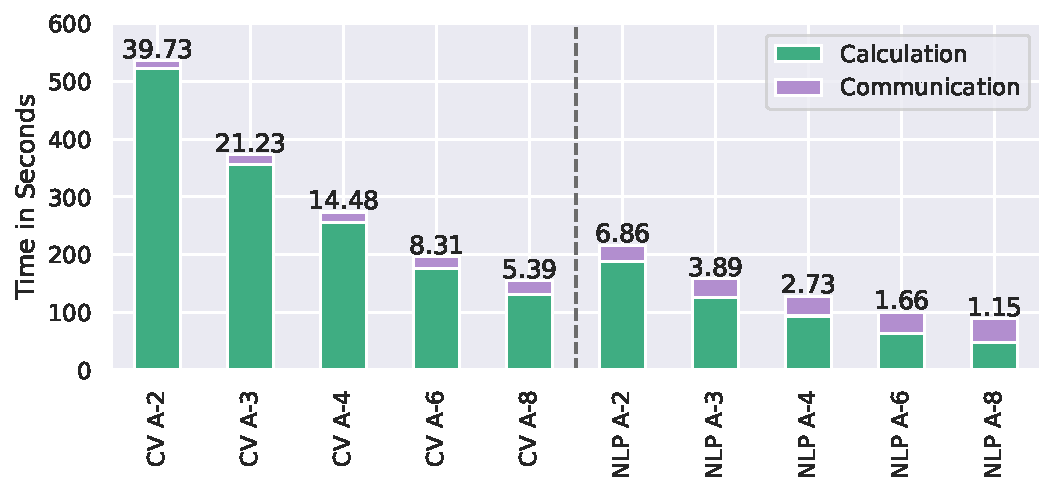
\includegraphics[width=\textwidth]{figures/misc/geo-distributed-performance-US-granularity}  
        \vspace{-18pt}
        \caption{Granularity}
        \label{fig:geo-dist-us-only-granularity}
    \end{subfigure}
    \vspace{-10pt}
    \caption{(A) Intra-zone performance for CV and NLP.}
    \label{fig:geo-dist-us-only}
    \vspace*{-5mm}
\end{figure}

The peak network bandwidth utilization between peers was at most a symmetric 1.1~Gbits while averaging and 33 Mbits ingress while training due to data loading.
This means that the network bandwidth of 7~Gbits was not a limiting factor.

\textbf{(B) Transatlantic scalability.} We scale when computing hardware is local. However, what happens when there is cheap capacity in another region? In this case, we study the throughput of experiments with resources in the \texttt{us-west} and \texttt{eu-central} regions (B-2,4,6,8 in ~\Cref{tab:geodistributed-experiments}).

The B-2 experiment has one VM in the US and one in the EU, achieving a virtually identical throughput of 68.4 (US-EU) versus 70.1 (US) at CV (\Cref{fig:geo-dist-us-eu-throughput}). 
Our maximum peak egress rate of 250~Mbits does not affect the CV experiments, while the US experiments peaked at 1.1 Gbits.
The reduction in bandwidth penalizes NLP harder, where we are 16\% slower with 177.3~SPS (US-EU) compared to the intra-zone experiment with 211.4~SPS (US).
The resulting increased communication can be easily seen in the granularity analysis in ~\Cref{fig:geo-dist-us-eu-granularity} (NLP A-2,4,6,8 vs. B-2,4,6,8).
As only communication time increases in the NLP \textbf{(B)} experiments compared to \textbf{(A)}, a granularity of $\gg1$ indicates good scalability: 
Adding two more GPUs to the B-6 experiment with a granularity of 1.03 results in a throughput increase of 15\% (B-8) relative to the baseline.
Meanwhile, adding two more GPUs to the B-2 experiment with a granularity of 2.21 results in a throughput increase of 77\% (B-4) relative to the baseline.

In the B-4 experiment, we look at what happens when we increase the number of VMs to four, with two in the US and two in the EU.
Nothing surprising happens with CV, as the workload continues to be mostly computation, with a throughput of 135.8 (B-4), only 3\% slower than the intra-zone experiment with 140.4 SPS (A-4).
However, at NLP, things get more interesting as we now have more overall communication with four peers, but they can average locally first and only later transmit across the Atlantic.
However, compared to their A-counterparts, we do not see a difference in relative scalability with either B-4, B-6, or B-8. % maybe talk a bit more in depth about the B-6 experiment where we have inbalanced compute?
This means that training across regions \textbf{(B)} is slower, but the contribution per GPU decreases at the same rate as in training within a zone \textbf{(A)}.
The per-GPU speedup with additional hardware reduces at the same rate for either setup (between 0.05 and 0.06).
This results in two observations: First, communication overhead scales linearly with the number of peers.
Second, we only have to pay the penalty for transatlantic training once.
However, we cannot expect a significant improvement in communication efficiency when we increase the amount of available local resources.

Summarizing, with an transatlantic setup, CV achieves a virtually identical maximum speedup of 3.2x with 8 GPUs compared to A-1 (B-8 is 2\% slower than A-8), while NLP is more affected by lower network bandwidth and only achieves a speedup of 2.15x (B-8 is 22\% slower than A-8).
The transatlantic training penalty is applied once;  however, it does not affect the relative scaling with additional compute resources.

\begin{figure}
    \begin{subfigure}[c]{0.25\textwidth}
        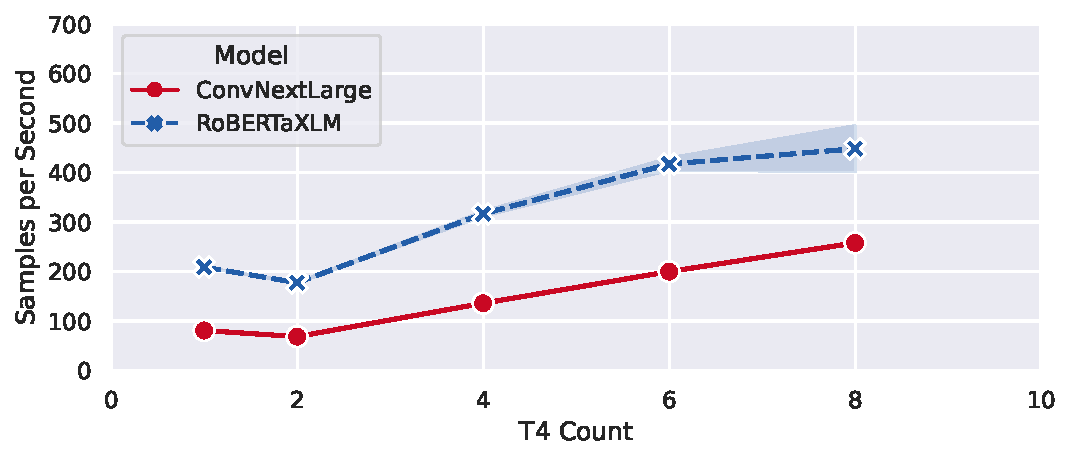
\includegraphics[width=\textwidth]{figures/misc/geo-distributed-performance-US-EU}
        \vspace{-15pt}
        \caption{Throughput}
        \label{fig:geo-dist-us-eu-throughput}
    \end{subfigure}
    \begin{subfigure}[c]{0.22\textwidth}
        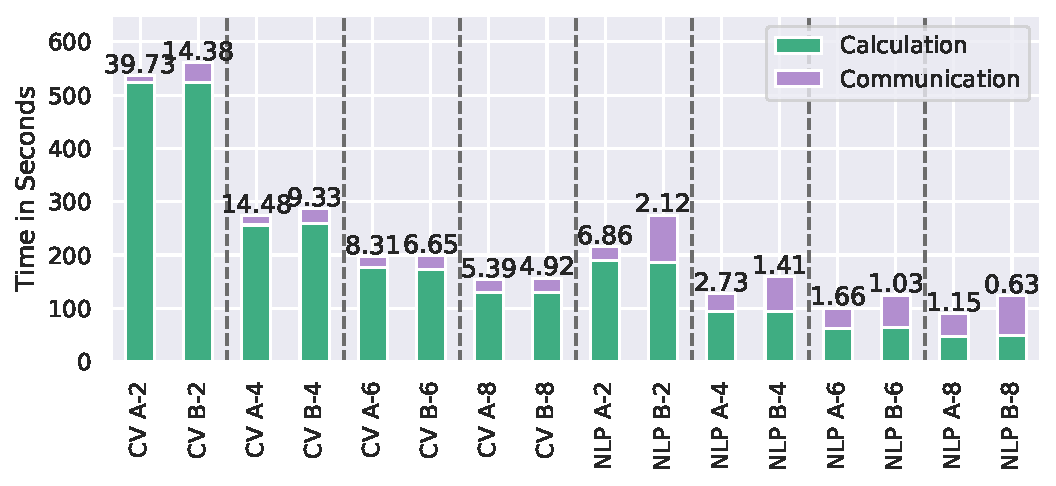
\includegraphics[width=\textwidth]{figures/misc/geo-distributed-performance-US-EU-granularity}  
        \vspace{-15pt}
        \caption{Granularity}
        \label{fig:geo-dist-us-eu-granularity}
    \end{subfigure}
    \vspace{-10pt}
    \caption{(B) Transatlantic performance for CV and NLP.}
    \label{fig:geo-dist-us-eu}
    \vspace*{-4mm}
\end{figure}
  
\textbf{(C) Intercontinental scalability. } To take geo-distribution to the extreme, we spawn VMs in up to 4 regions: USA, EU, ASIA, and AUS, to see how much worse bandwidth affects the training throughput (C-3,4,6,8 in ~\Cref{tab:geodistributed-experiments}).

\begin{figure}
    \begin{subfigure}[c]{0.25\textwidth}
        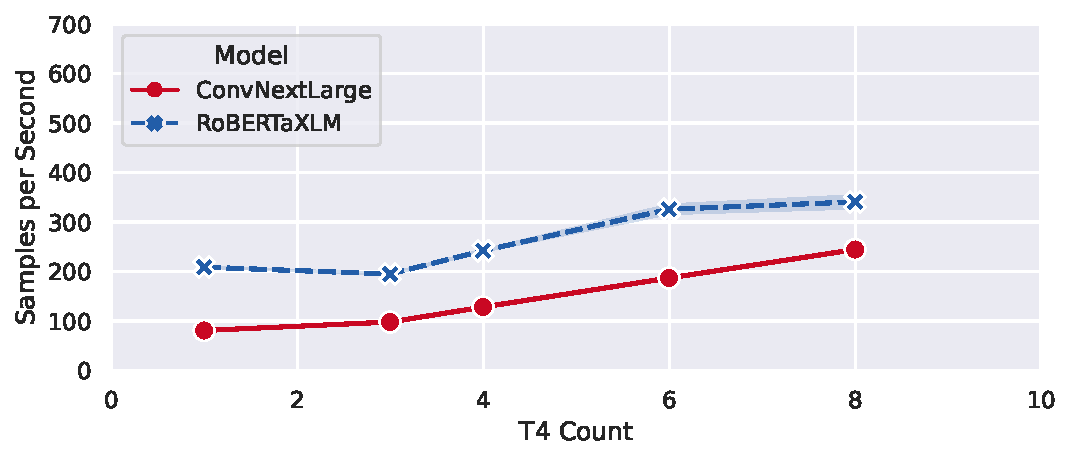
\includegraphics[width=\textwidth]{figures/misc/geo-distributed-performance-US-EU-ASIA-AUS}
        \vspace{-15pt}
        \caption{Throughput}
        \label{fig:geo-dist-us-eu-asia-aus-throughput}
    \end{subfigure}
    \begin{subfigure}[c]{0.22\textwidth}
        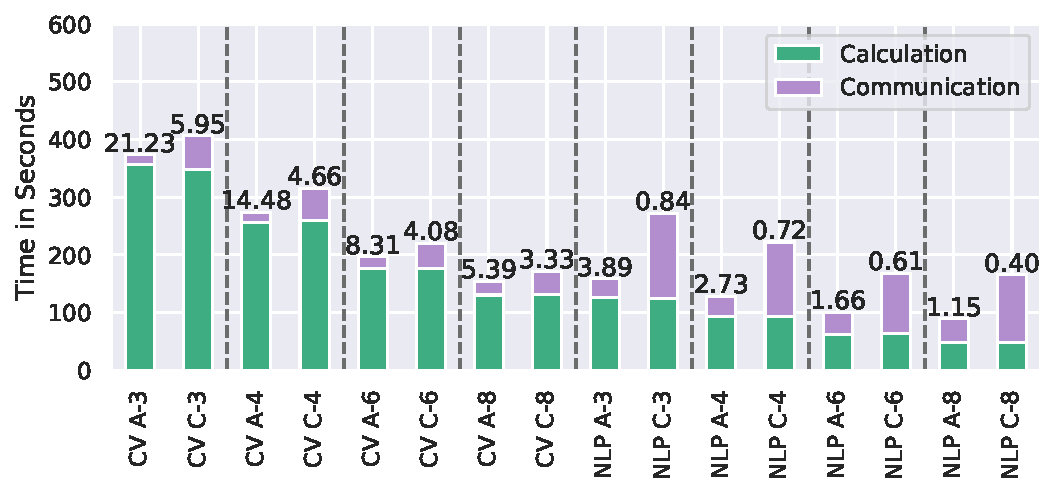
\includegraphics[width=\textwidth]{figures/misc/geo-distributed-performance-US-EU-ASIA-AUS-granularity}  
        \vspace{-15pt}
        \caption{Granularity}
        \label{fig:geo-dist-us-eu-asia-aus-granularity}
    \end{subfigure}
    \vspace{-10pt}
    \caption{(C) Intercontinental performance for CV and NLP.}
    \label{fig:geo-dist-us-eu-asia-oce}
    \vspace*{-7mm}
\end{figure} 

How does the intercontinental penalty investigated in \textbf{(B)} affect deployments with a single GPU on each continent?
Comparing the A-3 and C-3 experiments with three local versus three fully remote GPUs, CV is only 5\% slower, while NLP suffers a 34\% drop in throughput (\Cref{fig:geo-dist-us-eu-asia-aus-throughput}) and does not even reach the baseline single GPU performance (A-1).
The peak egress for each region was 318, 258, and 237 Mbits for the US, EU, and ASIA, respectively.
Since our bandwidth measurements were 210 and 130 Mbits from the US to the EU and ASIA, respectively (\Cref{tab:geodistributed-network}), this suggests that the averaging was done over the US node and not an N-to-N all-reduce (a detailed analysis of how averaging affects bandwidths is discussed in ~\Cref{sec:hybrid-cloud-performance}).
Thus, the limiting factor was the US-ASIA connection at 130 Mbits rather than the 80 Mbits from EU-ASIA.
The same trend continues with the C-4 run, which adds AUS as a continent with one additional VM.
As we know from the transatlantic experiments \textbf{(B)} that an additional continent has a detrimental effect on throughput, which, for the four continents experiment, C-4, results in a 9\% slower throughput for CV and 36\% slower for NLP compared to the A-4 runs (\Cref{fig:geo-dist-us-only-throughput}).
Again, the US VM is used as an averaging intermediary with a peak egress of 365 Mbits, while the other continents are between 318 and 330 Mbits.
When comparing the two continents (B-4) versus four continents (C-4) experiments, one GPU on each continent (C-4) is slower by 6\% for CV and 20\% for NLP compared to two GPUs on two continents (B-4).
This reinforces that local hardware should be preferred whenever possible.
However, we are always faster than the baseline (A-1), starting from 4 GPUs in both the transatlantic and intercontinental settings.
While these experiments were specifically designed to be a worst-case scenario, what about a more balanced GPU distribution with at least two GPUs in each region?

When comparing the C-6 experiment with two GPUs in three continents to the local A-6 experiments, the throughput slowdown is almost identical (CV 7\%, NLP 35\%) as with C-4 (CV 9\%, NLP 36\%) to A-4.
Scaling further to two GPUs in four continents, C-8 is slightly slower at NLP (41\%) compared to C-4 (36\%) to their respective local runs (A-8 and A-4), due to the decreasing granularity of 0.4 (\Cref{fig:geo-dist-us-eu-asia-aus-granularity}).
The small granularity removes the additional gain of four more GPUs since the task is no longer suitable for distributed training.
However, as the CV task is still at a granularity of 3.33 on C-8, it reaches a speedup of 3.02x, only 7\% slower than the fully local A-8 experiment.
The peak egress of 678 Mbits was also reached on one US VM, while the remaining VMs were between 450 and 550 Mbits.
These observations show that adding another continent does not significantly reduce throughput when training on three continents with at least two VMs to take advantage of the fast local connection, and the task granularity allows scaling.

In summary, while local compute is the best choice for maximum throughput, for high granularity tasks like CV, even distributing VMs over four continents only slows down performance by 7\%.
However, intercontinental training leads to a significant penalty on a task with lower granularity, like NLP, resulting in a performance drop of 41\% (C-8) compared to the fully local experiment (A-8).
Finally, each additional region introduces a constant penalty that is not amortized by adding local hardware, which should be considered when running geo-distributed training setups.